\question{Высокочастотный триод. Движение электронов в промежутке катод-сетка}

Аналогично предыдущему вопросу можно описать поведение электронов в промежутке
катод-сетка, если предположить, что вместо анода диода в плоскости \( z = d \)
находится сетка триода. Вместо анодного напряжения следует подразумевать
напряжение на сетке \( U_c = U_{c0}\sin\omega t + U_0 \).

Остановимся подробнее на процессах, происходящих при расстояниях катод-сетка,
близких к критическому \( d_\text{кр} \).

Для каждого положительного угла влета \( \omega t_k \) имеется максимальное
приведенное расстояние \( Z_{\max} \), которое достигает электрон за 1~период
высокочастотного поля (рис.~\pic{28Zmax}).

\begin{figure}[h!]
  \center
%  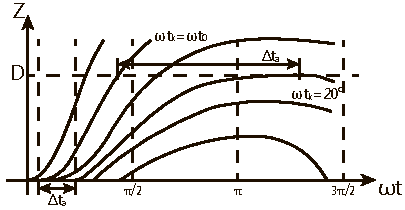
\includegraphics[width=.4\textwidth]{28_graph} \hspace{1em}
%  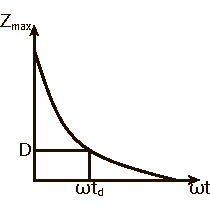
\includegraphics[width=.3\textwidth]{28_Z_max} \\
  \parbox{.4\textwidth}{\caption{Семейство кривых \( Z(\omega t) \)}
    \label{pic28graph}}
  \parbox{.35\textwidth}{\caption{Зависимость \( Z_{\max}(\omega t) \)}
    \label{pic28Zmax}}
\end{figure}

Если \( \omega t_0 > \omega t_d \), то ни один электрон не пересечет область
сетки. Если \( \omega t_0 < \omega t_d \), то часть электронов, эмитируемых в
промежуток фазы \( [\omega t_0, \omega t_d] \), проходит сетку и образует в
пространстве <<сетка-анод>> электронный импульс. Остальные электроны
возвращаются на катод, подогревая его и участвуя во вторичной эмиссии.

Определим заряд электронов, достигающих сетки в течение одного импульса, и заряд
электронов, возвращающихся на катод.
\begin{gather*}
  q_c = \frac{1}{\omega} \int\limits_{\omega t_0}^{\omega t_d} j_\text{э}\,
    d(\omega t) = \frac{\Ez}{\omega d} \int\limits_{\omega t_0}^{\omega t_d}
    \omega U_{c0}\cos\omega t\,d(\omega t) = \frac{\Ez U_{c0}}{d} \bigl(
    \sin\omega t_d - \sin\omega t_0 \big). \\
  q_\text{к} = \frac{1}{\omega} \int\limits_{\omega t_d}^{\pi / 2} j_\text{э}\,
    d(\omega t) = \frac{\Ez}{\omega d} \int\limits_{\omega t_d}^{\pi / 2}
    \omega U_{c0}\cos\omega t\,d(\omega t) = \frac{\Ez U_{c0}}{d} \bigl(1 -
    \sin\omega t_d \big).
\end{gather*}

Средние значение (постоянные составляющие) плотностей токов, проходящих через
сетку и возвращающихся на катод, равны, соответственно
\[
  j_{\text{э}c0} = \frac{q_c\omega}{2\pi} = \frac{U_{c0}\Ez\omega}{d}
    \big( \sin\omega t_d - \sin\omega t_0 \big), \quad
    j_{\text{эк}0} = \frac{q_\text{к}\omega}{2\pi} = \frac{U_{c0}\Ez\omega}{d}
    \big( 1 - \sin\omega t_d \big).
\]

Длительность импульса электронного тока, проходящего через сетку, больше, чем
время \( t_d - t_0 \). Это связано с тем, что скорость первых электронов выше,
чем скорость последующих. Данное явление носит название сеточного расширения
импульса. Форма импульса определяется из закона сохранения заряда:
\[
  j_\text{э}\,dt_\text{э} = j_c\,dt_c; \qquad
    j_c = j_\text{э} \left( \der{t_c}{t_\text{э}} \right)^{-1}.
\]
Производная \( \displaystyle \der{t_c}{t_\text{э}} \) определяется из графика на
рисунке~\pic{28graph}.

Полная кинетическая энергия, которую имеют электроны одного импульса при
пересечении единичной площадки сетки:
\[
  E_c = \int\frac{mv^2}{2} \frac{1}{S} \frac{dq}{e} = \int\limits_{t_0}^{t_d}
    \frac{mv^2}{2} \frac{j_\text{э}}{e}\,dt = \frac{m}{2e\omega}
    \int\limits_{\omega t_0}^{\omega t_d} v^2(\omega t) j_\text{э}\,
    d(\omega t).
\]

Средняя мощность, затрачиваемая источником питания и источником сигнала на
ускорение и формирование электронного импульса:
\[
  P_{c0} = \frac{E_c}{T} = \frac{E_c \omega}{2\pi}.
\]

Средняя мощность, затрачиваемая на возврат электронов, на нагрев катода и др.:
\[
  P_{\text{к}0} = \frac{m}{4e\pi}\int\limits_{\omega t_d}^{\pi / 2}
    v^2(\omega t) j_\text{э}\,d(\omega t).
\]

Полная мощность, затрачиваемая источником питания и источником сигнала
\(
  P_0 = P_{c0} + P_{\text{к}0}
\).
